\PassOptionsToPackage{unicode=true}{hyperref} % options for packages loaded elsewhere
\PassOptionsToPackage{hyphens}{url}
%
\documentclass[]{book}
\usepackage{lmodern}
\usepackage{amssymb,amsmath}
\usepackage{ifxetex,ifluatex}
\usepackage{fixltx2e} % provides \textsubscript
\ifnum 0\ifxetex 1\fi\ifluatex 1\fi=0 % if pdftex
  \usepackage[T1]{fontenc}
  \usepackage[utf8]{inputenc}
  \usepackage{textcomp} % provides euro and other symbols
\else % if luatex or xelatex
  \usepackage{unicode-math}
  \defaultfontfeatures{Ligatures=TeX,Scale=MatchLowercase}
\fi
% use upquote if available, for straight quotes in verbatim environments
\IfFileExists{upquote.sty}{\usepackage{upquote}}{}
% use microtype if available
\IfFileExists{microtype.sty}{%
\usepackage[]{microtype}
\UseMicrotypeSet[protrusion]{basicmath} % disable protrusion for tt fonts
}{}
\IfFileExists{parskip.sty}{%
\usepackage{parskip}
}{% else
\setlength{\parindent}{0pt}
\setlength{\parskip}{6pt plus 2pt minus 1pt}
}
\usepackage{hyperref}
\hypersetup{
            pdftitle={Parenting Under Pressure},
            pdfauthor={Bridget Callaghan, Kristen Chu, Emily Towner},
            pdfborder={0 0 0},
            breaklinks=true}
\urlstyle{same}  % don't use monospace font for urls
\usepackage{longtable,booktabs}
% Fix footnotes in tables (requires footnote package)
\IfFileExists{footnote.sty}{\usepackage{footnote}\makesavenoteenv{longtable}}{}
\usepackage{graphicx,grffile}
\makeatletter
\def\maxwidth{\ifdim\Gin@nat@width>\linewidth\linewidth\else\Gin@nat@width\fi}
\def\maxheight{\ifdim\Gin@nat@height>\textheight\textheight\else\Gin@nat@height\fi}
\makeatother
% Scale images if necessary, so that they will not overflow the page
% margins by default, and it is still possible to overwrite the defaults
% using explicit options in \includegraphics[width, height, ...]{}
\setkeys{Gin}{width=\maxwidth,height=\maxheight,keepaspectratio}
\setlength{\emergencystretch}{3em}  % prevent overfull lines
\providecommand{\tightlist}{%
  \setlength{\itemsep}{0pt}\setlength{\parskip}{0pt}}
\setcounter{secnumdepth}{5}
% Redefines (sub)paragraphs to behave more like sections
\ifx\paragraph\undefined\else
\let\oldparagraph\paragraph
\renewcommand{\paragraph}[1]{\oldparagraph{#1}\mbox{}}
\fi
\ifx\subparagraph\undefined\else
\let\oldsubparagraph\subparagraph
\renewcommand{\subparagraph}[1]{\oldsubparagraph{#1}\mbox{}}
\fi

% set default figure placement to htbp
\makeatletter
\def\fps@figure{htbp}
\makeatother

\usepackage{booktabs}
\usepackage{amsthm}
\makeatletter
\def\thm@space@setup{%
  \thm@preskip=8pt plus 2pt minus 4pt
  \thm@postskip=\thm@preskip
}
\makeatother
\usepackage[]{natbib}
\bibliographystyle{apalike}

\title{Parenting Under Pressure}
\author{Bridget Callaghan, Kristen Chu, Emily Towner}
\date{2021-09-29}

\begin{document}
\maketitle

{
\setcounter{tocdepth}{1}
\tableofcontents
}
\hypertarget{introduction}{%
\chapter{Introduction}\label{introduction}}

\begin{figure}
\centering

\includegraphics{images/PUP_header.png}
\caption{}
\end{figure}

The recent COVID-19 pandemic has caused tremendous pressure on caregivers, children, and families on a global scale. Previous research investigating the impacts of traumatic events on caregiver child relationships has shown the importance of maintaining positive caregiver child relationships in order to buffer the distress of the child. Despite the fact that traumatic events may present several challenges that potentially strain caregiver child relationships, parental buffering may alleviate anxiety and stress. While there is a breadth of existing research that encapsulates the benefits of strong caregiver child relationships during troubled times, little research exists on the transfer of parent threat information to children and its implications in the child's heightened fear and anxiety. Furthermore, few studies have surfaced regarding the larger emotional and behavioral impacts of COVID-19 on caregivers and children alike. As a traumatic experience, COVID-19 poses unique threats to families due its impacts in social distancing and self-isolation. Research in this topic will be integral to informing interventions that may diminish the negative effects of this traumatic experience for the future.

This study seeks to explore the ways in which the COVID-19 outbreak has specifically influenced caregivers, children, and families. In determining children's largest sources of information about COVID-19, we will assess the impacts of parent threat information on the child's fear about illness and contamination, and the larger implications for the child's anxiety. Moreover, we will evaluate the impacts of the COVID-19 outbreak on parent-child relationships and parental stress, focusing on the potential ways in which caregivers are buffering their child's stress during this period.

\textbf{Keywords}

Parenting, COVID-19, pandemic, stress, children

\begin{center}\rule{0.5\linewidth}{0.5pt}\end{center}

\hypertarget{summary}{%
\section{Summary}\label{summary}}

This study will be available in both English and Spanish. The study will gather both qualitative and quantitative data from parents and their children through an anonymous online questionnaire. The target population for this study will be parents with children aged 6-17 years old. The online survey is a mixed methods design and will include a multitude of questionnaires related to fear, anxiety, sleep, and parent child relationships prior to (retrospectively reported) and during the context of the COVID-19 outbreak.

\begin{center}\rule{0.5\linewidth}{0.5pt}\end{center}

\hypertarget{background}{%
\section{Background}\label{background}}

The effect of mass traumatic events has been shown to be extremely impactful to psychological health. Mass trauma experiences can result in a number of acute and chronic stress reactions, which may lead to a number of longer-term poor mental health outcomes (Chriman \& Dougherty, 2014). More specifically, previous outbreaks have been shown to cause tremendous impacts on fear, anxiety, depression, posttraumatic stress, and subjective well being (Cheng \& Cheuong, 2005; Perrin et al., 2009; Wu et al., 2005). While a large majority of the population may experience negative impacts on their mental health, caregivers and children may carry a specific set of challenges following such traumatic events.

Mass traumatic events disrupt a system of care and security, which may largely impact family relationships (Gerwitz et al., 2008). Not only are children particularly vulnerable to the threats posed by fearful events and subsequent pervasive media coverage (Pfefferbaum et al., 2005), but previous research in the context of terror attacks has shown that children are also largely affected by negative parental reactions to such events (Phillips et al., 2003). Negative parental reactions, which may root from a caregiver's own concerns about health, job security, their child's safety, was found to be associated with higher distress in children (Phillips et al., 2003).

Although each traumatic event may pose its own unique challenges and impacts, the impact of parent action to child outcome has been displayed in previous research regarding pandemics. Literature on the 2009 Swine Flu pandemic has assessed the role of parent threat information and its impacts on child fear of the pandemic, highlighting the significant relationship between parental fear of the disease and its transmission to child fear through parental sources of information (Remmerswaal \& Muris, 2011).

\begin{center}\rule{0.5\linewidth}{0.5pt}\end{center}

\hypertarget{specific-aims}{%
\section{Specific Aims}\label{specific-aims}}

The proposed study will assess the impacts of COVID-19 on caregiver-child relationships and mental health outcomes for children. This study has 4 specific aims:

\begin{enumerate}
\def\labelenumi{(\arabic{enumi})}
\tightlist
\item
  Determine the impacts of COVID-19 on caregiver-child relationships and parental stress.
\item
  Identify whether the transfer of parent threat information about COVID-19 is associated with higher fear and anxiety in children.
\item
  Determine whether parental buffering actions during COVID-19 can moderate the association between parent threat information and poorer mental health outcomes in children.
\item
  Establish underlying emotional themes within qualitative responses detailing COVID-19 experiences within the family unit.
\end{enumerate}

We hypothesize that parents who engage with more threat-related media and less buffering activities will have higher levels of parenting stress and children with higher levels of distress.

\hypertarget{methods}{%
\chapter{Methods}\label{methods}}

\hypertarget{rationale}{%
\section{Rationale}\label{rationale}}

Researchers separated PUP 1 (4/27/2020-5/28/2020; participant 159) and PUP 2 (5/29-7/30/2020, participant 324). PUP 2 incorporated a Spanish collection (7/8/2020-7/30/2020).

\hypertarget{pup-1-measures}{%
\section{PUP 1 Measures}\label{pup-1-measures}}

\hypertarget{information}{%
\subsection{Information}\label{information}}

\begin{longtable}[]{@{}llll@{}}
\toprule
\begin{minipage}[b]{0.13\columnwidth}\raggedright
Title\strut
\end{minipage} & \begin{minipage}[b]{0.21\columnwidth}\raggedright
Name\strut
\end{minipage} & \begin{minipage}[b]{0.31\columnwidth}\raggedright
Description\strut
\end{minipage} & \begin{minipage}[b]{0.23\columnwidth}\raggedright
Reference\strut
\end{minipage}\tabularnewline
\midrule
\endhead
\begin{minipage}[t]{0.13\columnwidth}\raggedright
information\strut
\end{minipage} & \begin{minipage}[t]{0.21\columnwidth}\raggedright
COVID-19 Information\strut
\end{minipage} & \begin{minipage}[t]{0.31\columnwidth}\raggedright
This questionnaire identifies information regarding how many children participants have and demographic information regarding the household.\strut
\end{minipage} & \begin{minipage}[t]{0.23\columnwidth}\raggedright
Made by BABLab\strut
\end{minipage}\tabularnewline
\begin{minipage}[t]{0.13\columnwidth}\raggedright
covid\_objective\strut
\end{minipage} & \begin{minipage}[t]{0.21\columnwidth}\raggedright
COVID-19 Objective\strut
\end{minipage} & \begin{minipage}[t]{0.31\columnwidth}\raggedright
This questionnaire identifies health changes from the impacts of the COVID-19 outbreak.\strut
\end{minipage} & \begin{minipage}[t]{0.23\columnwidth}\raggedright
Made by BABLab; adapted from the CASPE- parent (Lacouceur, 2020), the Combined COVID Health Emotional Lifestyle Changes (Pfiefer, 2020), and the COVID Lifestyle Changes (Pfiefer, 2020)\strut
\end{minipage}\tabularnewline
\begin{minipage}[t]{0.13\columnwidth}\raggedright
demographics\strut
\end{minipage} & \begin{minipage}[t]{0.21\columnwidth}\raggedright
Demographics\strut
\end{minipage} & \begin{minipage}[t]{0.31\columnwidth}\raggedright
This questionnaire consists of 23 items to identify the child's age, caregiver information, parental socioeconomic status, underlying health conditions, and geographic location. This questionnaire also contains the MacArthur Scale of Subjective Social Status, which assesses the sense of social status across factors of socioeconomic status by asking individuals to place an ``X'' on the area of the ``social ladder'' they feel they most identify.\strut
\end{minipage} & \begin{minipage}[t]{0.23\columnwidth}\raggedright
(Adler et al., 2000)\strut
\end{minipage}\tabularnewline
\bottomrule
\end{longtable}

\hypertarget{affect}{%
\subsection{Affect}\label{affect}}

\begin{longtable}[]{@{}llll@{}}
\toprule
\begin{minipage}[b]{0.13\columnwidth}\raggedright
Title\strut
\end{minipage} & \begin{minipage}[b]{0.21\columnwidth}\raggedright
Name\strut
\end{minipage} & \begin{minipage}[b]{0.38\columnwidth}\raggedright
Description\strut
\end{minipage} & \begin{minipage}[b]{0.15\columnwidth}\raggedright
Reference\strut
\end{minipage}\tabularnewline
\midrule
\endhead
\begin{minipage}[t]{0.13\columnwidth}\raggedright
PANAS\strut
\end{minipage} & \begin{minipage}[t]{0.21\columnwidth}\raggedright
Positive and Negative Affect Schedule- Parent Self-Report\strut
\end{minipage} & \begin{minipage}[t]{0.38\columnwidth}\raggedright
This self-report questionnaire consists of 20 items measuring both positive and negative affect. The questionnaire asks participants to rate each item on a 5-point scale of 1 (not at all) to 5 (very much) indicating the way they have felt over the past week.\strut
\end{minipage} & \begin{minipage}[t]{0.15\columnwidth}\raggedright
(Watson et al., 1988)\strut
\end{minipage}\tabularnewline
\begin{minipage}[t]{0.13\columnwidth}\raggedright
Written Reponse\strut
\end{minipage} & \begin{minipage}[t]{0.21\columnwidth}\raggedright
COVID-19 Written Response- Parent\strut
\end{minipage} & \begin{minipage}[t]{0.38\columnwidth}\raggedright
This self-report measure consists of one long-form qualitative response, prompting a parent to write continuously for five minutes about the impacts of COVID-19 on their life and family.\strut
\end{minipage} & \begin{minipage}[t]{0.15\columnwidth}\raggedright
Made by BABLab; adapted from (Pennebaker, 1997)\strut
\end{minipage}\tabularnewline
\bottomrule
\end{longtable}

\hypertarget{anxiety}{%
\subsection{Anxiety}\label{anxiety}}

\begin{longtable}[]{@{}llll@{}}
\toprule
\begin{minipage}[b]{0.13\columnwidth}\raggedright
Title\strut
\end{minipage} & \begin{minipage}[b]{0.21\columnwidth}\raggedright
Name\strut
\end{minipage} & \begin{minipage}[b]{0.38\columnwidth}\raggedright
Description\strut
\end{minipage} & \begin{minipage}[b]{0.15\columnwidth}\raggedright
Reference\strut
\end{minipage}\tabularnewline
\midrule
\endhead
\begin{minipage}[t]{0.13\columnwidth}\raggedright
RCADS--P\strut
\end{minipage} & \begin{minipage}[t]{0.21\columnwidth}\raggedright
Revised Children's Anxiety and Depression Scale--Parent Proxy\strut
\end{minipage} & \begin{minipage}[t]{0.38\columnwidth}\raggedright
This 47 item questionnaire contains subscales of separation anxiety disorder, social phobia, panic disorder, low mood, obsessive compulsive disorder, and generalized anxiety disorder. The scale asks participants to rate how often their child experiences each item.\strut
\end{minipage} & \begin{minipage}[t]{0.15\columnwidth}\raggedright
(Chorpita et al., 2000)\strut
\end{minipage}\tabularnewline
\begin{minipage}[t]{0.13\columnwidth}\raggedright
STAI\strut
\end{minipage} & \begin{minipage}[t]{0.21\columnwidth}\raggedright
Shortened State-Trait Anxiety Inventory-Parent Self-Report\strut
\end{minipage} & \begin{minipage}[t]{0.38\columnwidth}\raggedright
This Inventory contains a shortened State-Trait Anxiety Inventory, with 6 total items detailing state anxiety. The inventory asks participants to rate how often they feel each item, in the context of how the participant feels currently.\strut
\end{minipage} & \begin{minipage}[t]{0.15\columnwidth}\raggedright
(Spielberger et al., 1983)\strut
\end{minipage}\tabularnewline
\bottomrule
\end{longtable}

\hypertarget{early-life-stress}{%
\subsection{Early Life Stress}\label{early-life-stress}}

\begin{longtable}[]{@{}llll@{}}
\toprule
\begin{minipage}[b]{0.13\columnwidth}\raggedright
Title\strut
\end{minipage} & \begin{minipage}[b]{0.21\columnwidth}\raggedright
Name\strut
\end{minipage} & \begin{minipage}[b]{0.38\columnwidth}\raggedright
Description\strut
\end{minipage} & \begin{minipage}[b]{0.15\columnwidth}\raggedright
Reference\strut
\end{minipage}\tabularnewline
\midrule
\endhead
\begin{minipage}[t]{0.13\columnwidth}\raggedright
TESI-PRR\strut
\end{minipage} & \begin{minipage}[t]{0.21\columnwidth}\raggedright
Traumatic Events Screening Inventory - Parent Report Revised\strut
\end{minipage} & \begin{minipage}[t]{0.38\columnwidth}\raggedright
The TESI-PRR assesses a child's/adolescent's experience of a variety of potential traumatic events including previous injuries, hospitalizations, domestic violence, community violence, disasters, accidents, abuse.\strut
\end{minipage} & \begin{minipage}[t]{0.15\columnwidth}\raggedright
(Ghosh-Ippen et al., 2002)\strut
\end{minipage}\tabularnewline
\bottomrule
\end{longtable}

\hypertarget{fear}{%
\subsection{Fear}\label{fear}}

\begin{longtable}[]{@{}llll@{}}
\toprule
\begin{minipage}[b]{0.13\columnwidth}\raggedright
Title\strut
\end{minipage} & \begin{minipage}[b]{0.21\columnwidth}\raggedright
Name\strut
\end{minipage} & \begin{minipage}[b]{0.38\columnwidth}\raggedright
Description\strut
\end{minipage} & \begin{minipage}[b]{0.15\columnwidth}\raggedright
Reference\strut
\end{minipage}\tabularnewline
\midrule
\endhead
\begin{minipage}[t]{0.13\columnwidth}\raggedright
FIVE-Parent Report\strut
\end{minipage} & \begin{minipage}[t]{0.21\columnwidth}\raggedright
Fear of Illness and Virus Evaluation- Parent Proxy Report\strut
\end{minipage} & \begin{minipage}[t]{0.38\columnwidth}\raggedright
This is a 35-item parent report questionnaire constructed to measure child fear of illness and virus. This questionnaire lists items related to fears about contamination, illness, and social distancing, and behaviors and impacts related to these illness and virus fears and asks participants to rate on a scale of 1-4 how often they are afraid of each item within the last week.\strut
\end{minipage} & \begin{minipage}[t]{0.15\columnwidth}\raggedright
(Ehrenreich-May, 2020)\strut
\end{minipage}\tabularnewline
\begin{minipage}[t]{0.13\columnwidth}\raggedright
FIVE- Adult Report\strut
\end{minipage} & \begin{minipage}[t]{0.21\columnwidth}\raggedright
Fear of Illness and Virus Evaluation- Parent Self-Report\strut
\end{minipage} & \begin{minipage}[t]{0.38\columnwidth}\raggedright
This is a 35-item parent report questionnaire constructed to measure adult fear of illness and virus. This questionnaire lists items related to fears about contamination, illness, and social distancing, and behaviors and impacts related to these illness and virus fears and asks participants to rate on a scale of 1-4 how often they are afraid of each item within the last week.\strut
\end{minipage} & \begin{minipage}[t]{0.15\columnwidth}\raggedright
(Ehrenreich-May, 2020)\strut
\end{minipage}\tabularnewline
\begin{minipage}[t]{0.13\columnwidth}\raggedright
GMF-PR\strut
\end{minipage} & \begin{minipage}[t]{0.21\columnwidth}\raggedright
General Medical Fears Questionnaire- Parent Proxy Report\strut
\end{minipage} & \begin{minipage}[t]{0.38\columnwidth}\raggedright
This 7-item questionnaire is designed to evaluate child general medical fear. The measure asks participants to rate each item on a scale of 1-3 how much they fear each item.\strut
\end{minipage} & \begin{minipage}[t]{0.15\columnwidth}\raggedright
Made by BABLab; adapted from the Revised Fear Survey Schedule for Children (FSSC-R) (Ollendick, 1983)\strut
\end{minipage}\tabularnewline
\begin{minipage}[t]{0.13\columnwidth}\raggedright
GMF-SR\strut
\end{minipage} & \begin{minipage}[t]{0.21\columnwidth}\raggedright
General Medical Fears Questionnaire- Parent Self-Report\strut
\end{minipage} & \begin{minipage}[t]{0.38\columnwidth}\raggedright
This 7-item questionnaire is designed to evaluate parent general medical fear. The measure asks participants to rate each item on a scale of 1-3 how much they fear each item.\strut
\end{minipage} & \begin{minipage}[t]{0.15\columnwidth}\raggedright
Made by BABLab; adapted from the FSSC-R (Ollendick, 1983)\strut
\end{minipage}\tabularnewline
\bottomrule
\end{longtable}

\hypertarget{parent-child-relationship}{%
\subsection{Parent-Child Relationship}\label{parent-child-relationship}}

\begin{longtable}[]{@{}llll@{}}
\toprule
\begin{minipage}[b]{0.14\columnwidth}\raggedright
Title\strut
\end{minipage} & \begin{minipage}[b]{0.18\columnwidth}\raggedright
Name\strut
\end{minipage} & \begin{minipage}[b]{0.20\columnwidth}\raggedright
Description\strut
\end{minipage} & \begin{minipage}[b]{0.37\columnwidth}\raggedright
Reference\strut
\end{minipage}\tabularnewline
\midrule
\endhead
\begin{minipage}[t]{0.14\columnwidth}\raggedright
PCRQ\strut
\end{minipage} & \begin{minipage}[t]{0.18\columnwidth}\raggedright
Parent Child Relationship Questionnaire- Parent Report Form\strut
\end{minipage} & \begin{minipage}[t]{0.20\columnwidth}\raggedright
This is a 27-item questionnaire designed to measure the quality and security of the parent and child relationship. The questionnaire asks participants to rate on a scale of 1-5 how much each statement applies to him/her.\strut
\end{minipage} & \begin{minipage}[t]{0.37\columnwidth}\raggedright
Made by BABLab; adapted from the Emotional Availability Self Report (Biringen et al., 1998), Network of Relationships Inventory (Furman \& Buhrmester, 2009), Parental Reflective Functioning Questionnaire (Luyten, et al., 2017), Parent Emotion Regulation Scale (Pereira et al., 2017), Child Parent Relationship Scale (Pianta, 1992), and the Attachment Q-Sort Observational Measure (Waters \& Deane, 1985)\strut
\end{minipage}\tabularnewline
\bottomrule
\end{longtable}

\hypertarget{parental-buffering}{%
\subsection{Parental Buffering}\label{parental-buffering}}

\begin{longtable}[]{@{}llll@{}}
\toprule
\begin{minipage}[b]{0.14\columnwidth}\raggedright
Title\strut
\end{minipage} & \begin{minipage}[b]{0.22\columnwidth}\raggedright
Name\strut
\end{minipage} & \begin{minipage}[b]{0.31\columnwidth}\raggedright
Description\strut
\end{minipage} & \begin{minipage}[b]{0.22\columnwidth}\raggedright
Reference\strut
\end{minipage}\tabularnewline
\midrule
\endhead
\begin{minipage}[t]{0.14\columnwidth}\raggedright
PBQ\strut
\end{minipage} & \begin{minipage}[t]{0.22\columnwidth}\raggedright
Parental Buffering Questionnaire- Parent Report Form\strut
\end{minipage} & \begin{minipage}[t]{0.31\columnwidth}\raggedright
This questionnaire contains three blocks to assess parental buffering in child stress. The first block contains 6 items to assess parental belief in being effective buffers, prompting participants to rate on a scale of 1-7 to which they agree or disagree. The second block contains 15 items of buffering actions, with a scale of 1-7 measuring how often these actions occur and a scale of 1- 6 measuring effectiveness of each action. The third block contains a qualitative response about parent buffering of child stress.\strut
\end{minipage} & \begin{minipage}[t]{0.22\columnwidth}\raggedright
Made by BABLab; adapted from the Early Intervention Parenting Self-Efficacy Scale (Guimond et al., 2008), CASPE-Parent (Lacouceur, 2020), PERS (Pereira et al., 2017), and the Modified KIDCOPE (Pfiefer \& Lewis, 2020)\strut
\end{minipage}\tabularnewline
\begin{minipage}[t]{0.14\columnwidth}\raggedright
BIQ\strut
\end{minipage} & \begin{minipage}[t]{0.22\columnwidth}\raggedright
Buffering Information Questionnaire- Parent Proxy Form\strut
\end{minipage} & \begin{minipage}[t]{0.31\columnwidth}\raggedright
This 2 item questionnaire assesses whether parents feel they have access to adequate information to support their child's psychological health during COVID-19 and the sources of this information.\strut
\end{minipage} & \begin{minipage}[t]{0.22\columnwidth}\raggedright
Made by BABLab\strut
\end{minipage}\tabularnewline
\bottomrule
\end{longtable}

\hypertarget{parenting-stress}{%
\subsection{Parenting Stress}\label{parenting-stress}}

\begin{longtable}[]{@{}llll@{}}
\toprule
\begin{minipage}[b]{0.12\columnwidth}\raggedright
Title\strut
\end{minipage} & \begin{minipage}[b]{0.19\columnwidth}\raggedright
Name\strut
\end{minipage} & \begin{minipage}[b]{0.32\columnwidth}\raggedright
Description\strut
\end{minipage} & \begin{minipage}[b]{0.25\columnwidth}\raggedright
Reference\strut
\end{minipage}\tabularnewline
\midrule
\endhead
\begin{minipage}[t]{0.12\columnwidth}\raggedright
PSCQ\strut
\end{minipage} & \begin{minipage}[t]{0.19\columnwidth}\raggedright
Parenting Stress Covid-19 Questionnaire - Parent Report Form\strut
\end{minipage} & \begin{minipage}[t]{0.32\columnwidth}\raggedright
his questionnaire consists of two blocks, separating the evaluation of parental stress prior to COVID-19 with 4 items, and during COVID-19 with 6 items. The questionnaire asks participants to rate on a scale of 1-5 how much they agree with each item related to parental stress.\strut
\end{minipage} & \begin{minipage}[t]{0.25\columnwidth}\raggedright
Made by BABLab; adapted from the Parental Stress Scale (Berry \& Jones, 1995), COVID-19 Adolescent Symptom \& Psychological Experience Questionnaire- Parent (Ladouceur, 2020), and the Adolescent Social Connection \& Coping During COVID-19 Questionnaire (Pfiefer, 2020)\strut
\end{minipage}\tabularnewline
\begin{minipage}[t]{0.12\columnwidth}\raggedright
RDAS\strut
\end{minipage} & \begin{minipage}[t]{0.19\columnwidth}\raggedright
Revised Dyadic Adjustment Scale\strut
\end{minipage} & \begin{minipage}[t]{0.32\columnwidth}\raggedright
Used to assess the quality of the parents' relationship (if applicable). 14-item self report questionnaire that assesses seven dimensions of couple relationships within three overarching categories including ``Consensus'' in decision making, values and affection, ``Satisfaction'' in the relationship with respect to stability and conflict regulation, and ``Cohesion'' as seen through activities and discussion. Respondents rate certain aspects of their relationship on a 5 or 6 point scale.\strut
\end{minipage} & \begin{minipage}[t]{0.25\columnwidth}\raggedright
(Busby et al., 1995)\strut
\end{minipage}\tabularnewline
\bottomrule
\end{longtable}

\hypertarget{threat-information}{%
\subsection{Threat Information}\label{threat-information}}

\begin{longtable}[]{@{}llll@{}}
\toprule
\begin{minipage}[b]{0.14\columnwidth}\raggedright
Title\strut
\end{minipage} & \begin{minipage}[b]{0.23\columnwidth}\raggedright
Name\strut
\end{minipage} & \begin{minipage}[b]{0.27\columnwidth}\raggedright
Description\strut
\end{minipage} & \begin{minipage}[b]{0.25\columnwidth}\raggedright
Reference\strut
\end{minipage}\tabularnewline
\midrule
\endhead
\begin{minipage}[t]{0.14\columnwidth}\raggedright
SOI\strut
\end{minipage} & \begin{minipage}[t]{0.23\columnwidth}\raggedright
Sources of Information about COVID-19 Scale- Parent Proxy Report\strut
\end{minipage} & \begin{minipage}[t]{0.27\columnwidth}\raggedright
his 9-item questionnaire is designed to evaluate the sources of information in which children are receiving about COVID-19. The scale lists items related to parent threat information, media, school, friends and asks participants to rate on a scale of 1-5 how true each item about the source of information their child receives.\strut
\end{minipage} & \begin{minipage}[t]{0.25\columnwidth}\raggedright
Made by BABLab; adapted from the Sources of Information about Swine Flu Scale (Remmerswaal \& Muris, 2011)\strut
\end{minipage}\tabularnewline
\bottomrule
\end{longtable}

\begin{center}\rule{0.5\linewidth}{0.5pt}\end{center}

\hypertarget{pup-2-measures}{%
\section{PUP 2 Measures}\label{pup-2-measures}}

\hypertarget{information-1}{%
\subsection{Information}\label{information-1}}

\begin{longtable}[]{@{}llll@{}}
\toprule
\begin{minipage}[b]{0.14\columnwidth}\raggedright
Title\strut
\end{minipage} & \begin{minipage}[b]{0.22\columnwidth}\raggedright
Name\strut
\end{minipage} & \begin{minipage}[b]{0.30\columnwidth}\raggedright
Description\strut
\end{minipage} & \begin{minipage}[b]{0.24\columnwidth}\raggedright
Reference\strut
\end{minipage}\tabularnewline
\midrule
\endhead
\begin{minipage}[t]{0.14\columnwidth}\raggedright
information\strut
\end{minipage} & \begin{minipage}[t]{0.22\columnwidth}\raggedright
COVID-19 Information\strut
\end{minipage} & \begin{minipage}[t]{0.30\columnwidth}\raggedright
This questionnaire identifies information regarding how many children participants have and demographic information regarding the household.\strut
\end{minipage} & \begin{minipage}[t]{0.24\columnwidth}\raggedright
Made by BABLab\strut
\end{minipage}\tabularnewline
\begin{minipage}[t]{0.14\columnwidth}\raggedright
covid\_objective\strut
\end{minipage} & \begin{minipage}[t]{0.22\columnwidth}\raggedright
COVID-19 Objective\strut
\end{minipage} & \begin{minipage}[t]{0.30\columnwidth}\raggedright
This questionnaire identifies health changes from the impacts of the COVID-19 outbreak.\strut
\end{minipage} & \begin{minipage}[t]{0.24\columnwidth}\raggedright
Made by BABLab; adapted from the CASPE- parent (Lacouceur, 2020), the Combined COVID Health Emotional Lifestyle Changes (Pfiefer, 2020), and the COVID Lifestyle Changes (Pfiefer, 2020)\strut
\end{minipage}\tabularnewline
\begin{minipage}[t]{0.14\columnwidth}\raggedright
demographics\strut
\end{minipage} & \begin{minipage}[t]{0.22\columnwidth}\raggedright
Demographics\strut
\end{minipage} & \begin{minipage}[t]{0.30\columnwidth}\raggedright
This questionnaire consists of 23 items to identify the child's age, caregiver information, parental socioeconomic status, underlying health conditions, and geographic location. This questionnaire also contains the MacArthur Scale of Subjective Social Status, which assesses the sense of social status across factors of socioeconomic status by asking individuals to place an ``X'' on the area of the ``social ladder'' they feel they most identify.\strut
\end{minipage} & \begin{minipage}[t]{0.24\columnwidth}\raggedright
(Adler et al., 2000)\strut
\end{minipage}\tabularnewline
\bottomrule
\end{longtable}

\hypertarget{fear-1}{%
\subsection{Fear}\label{fear-1}}

\begin{longtable}[]{@{}llll@{}}
\toprule
\begin{minipage}[b]{0.13\columnwidth}\raggedright
Title\strut
\end{minipage} & \begin{minipage}[b]{0.21\columnwidth}\raggedright
Name\strut
\end{minipage} & \begin{minipage}[b]{0.38\columnwidth}\raggedright
Description\strut
\end{minipage} & \begin{minipage}[b]{0.15\columnwidth}\raggedright
Reference\strut
\end{minipage}\tabularnewline
\midrule
\endhead
\begin{minipage}[t]{0.13\columnwidth}\raggedright
FIVE-Parent Report\strut
\end{minipage} & \begin{minipage}[t]{0.21\columnwidth}\raggedright
Fear of Illness and Virus Evaluation- Parent Proxy Report\strut
\end{minipage} & \begin{minipage}[t]{0.38\columnwidth}\raggedright
This is a 35-item parent report questionnaire constructed to measure child fear of illness and virus. This questionnaire lists items related to fears about contamination, illness, and social distancing, and behaviors and impacts related to these illness and virus fears and asks participants to rate on a scale of 1-4 how often they are afraid of each item within the last week.\strut
\end{minipage} & \begin{minipage}[t]{0.15\columnwidth}\raggedright
(Ehrenreich-May, 2020)\strut
\end{minipage}\tabularnewline
\begin{minipage}[t]{0.13\columnwidth}\raggedright
FIVE- Adult Report\strut
\end{minipage} & \begin{minipage}[t]{0.21\columnwidth}\raggedright
Fear of Illness and Virus Evaluation- Parent Self-Report\strut
\end{minipage} & \begin{minipage}[t]{0.38\columnwidth}\raggedright
This is a 35-item parent report questionnaire constructed to measure adult fear of illness and virus. This questionnaire lists items related to fears about contamination, illness, and social distancing, and behaviors and impacts related to these illness and virus fears and asks participants to rate on a scale of 1-4 how often they are afraid of each item within the last week.\strut
\end{minipage} & \begin{minipage}[t]{0.15\columnwidth}\raggedright
(Ehrenreich-May, 2020)\strut
\end{minipage}\tabularnewline
\bottomrule
\end{longtable}

\hypertarget{parent-child-relationship-1}{%
\subsection{Parent-Child Relationship}\label{parent-child-relationship-1}}

\begin{longtable}[]{@{}llll@{}}
\toprule
\begin{minipage}[b]{0.14\columnwidth}\raggedright
Title\strut
\end{minipage} & \begin{minipage}[b]{0.18\columnwidth}\raggedright
Name\strut
\end{minipage} & \begin{minipage}[b]{0.24\columnwidth}\raggedright
Description\strut
\end{minipage} & \begin{minipage}[b]{0.33\columnwidth}\raggedright
Reference\strut
\end{minipage}\tabularnewline
\midrule
\endhead
\begin{minipage}[t]{0.14\columnwidth}\raggedright
PCRQ\strut
\end{minipage} & \begin{minipage}[t]{0.18\columnwidth}\raggedright
Parent Child Relationship Questionnaire- Parent Report Form\strut
\end{minipage} & \begin{minipage}[t]{0.24\columnwidth}\raggedright
This is a 27-item questionnaire designed to measure the quality and security of the parent and child relationship. The questionnaire asks participants to rate on a scale of 1-5 how much each statement applies to him/her.\strut
\end{minipage} & \begin{minipage}[t]{0.33\columnwidth}\raggedright
Made by BABLab; adapted from the Emotional Availability Self Report (Biringen et al., 1998), Network of Relationships Inventory (Furman \& Buhrmester, 2009), Parental Reflective Functioning Questionnaire (Luyten, et al., 2017), Parent Emotion Regulation Scale (Pereira et al., 2017), Child Parent Relationship Scale (Pianta, 1992), and the Attachment Q-Sort Observational Measure (Waters \& Deane, 1985)\strut
\end{minipage}\tabularnewline
\bottomrule
\end{longtable}

\hypertarget{parental-buffering-1}{%
\subsection{Parental Buffering}\label{parental-buffering-1}}

\begin{longtable}[]{@{}llll@{}}
\toprule
\begin{minipage}[b]{0.13\columnwidth}\raggedright
Title\strut
\end{minipage} & \begin{minipage}[b]{0.21\columnwidth}\raggedright
Name\strut
\end{minipage} & \begin{minipage}[b]{0.33\columnwidth}\raggedright
Description\strut
\end{minipage} & \begin{minipage}[b]{0.21\columnwidth}\raggedright
Reference\strut
\end{minipage}\tabularnewline
\midrule
\endhead
\begin{minipage}[t]{0.13\columnwidth}\raggedright
PBQ\strut
\end{minipage} & \begin{minipage}[t]{0.21\columnwidth}\raggedright
Parental Buffering Questionnaire- Parent Report Form\strut
\end{minipage} & \begin{minipage}[t]{0.33\columnwidth}\raggedright
This questionnaire contains three blocks to assess parental buffering in child stress. The first block contains 6 items to assess parental belief in being effective buffers, prompting participants to rate on a scale of 1-7 to which they agree or disagree. The second block contains 15 items of buffering actions, with a scale of 1-7 measuring how often these actions occur and a scale of 1- 6 measuring effectiveness of each action. The third block contains a qualitative response about parent buffering of child stress.\strut
\end{minipage} & \begin{minipage}[t]{0.21\columnwidth}\raggedright
Made by BABLab; adapted from the Early Intervention Parenting Self-Efficacy Scale (Guimond et al., 2008), CASPE-Parent (Lacouceur, 2020), PERS (Pereira et al., 2017), and the Modified KIDCOPE (Pfiefer \& Lewis, 2020)\strut
\end{minipage}\tabularnewline
\begin{minipage}[t]{0.13\columnwidth}\raggedright
BIQ\strut
\end{minipage} & \begin{minipage}[t]{0.21\columnwidth}\raggedright
Buffering Information Questionnaire- Parent Proxy Form\strut
\end{minipage} & \begin{minipage}[t]{0.33\columnwidth}\raggedright
This 2 item questionnaire assesses whether parents feel they have access to adequate information to support their child's psychological health during COVID-19 and the sources of this information.\strut
\end{minipage} & \begin{minipage}[t]{0.21\columnwidth}\raggedright
Made by BABLab\strut
\end{minipage}\tabularnewline
\bottomrule
\end{longtable}

\hypertarget{threat-information-1}{%
\subsection{Threat Information}\label{threat-information-1}}

\begin{longtable}[]{@{}llll@{}}
\toprule
\begin{minipage}[b]{0.13\columnwidth}\raggedright
Title\strut
\end{minipage} & \begin{minipage}[b]{0.21\columnwidth}\raggedright
Name\strut
\end{minipage} & \begin{minipage}[b]{0.38\columnwidth}\raggedright
Description\strut
\end{minipage} & \begin{minipage}[b]{0.15\columnwidth}\raggedright
Reference\strut
\end{minipage}\tabularnewline
\midrule
\endhead
\begin{minipage}[t]{0.13\columnwidth}\raggedright
SOI\strut
\end{minipage} & \begin{minipage}[t]{0.21\columnwidth}\raggedright
Sources of Information about COVID-19 Scale- Parent Proxy Report\strut
\end{minipage} & \begin{minipage}[t]{0.38\columnwidth}\raggedright
his 9-item questionnaire is designed to evaluate the sources of information in which children are receiving about COVID-19. The scale lists items related to parent threat information, media, school, friends and asks participants to rate on a scale of 1-5 how true each item about the source of information their child receives.\strut
\end{minipage} & \begin{minipage}[t]{0.15\columnwidth}\raggedright
Made by BABLab; adapted from the Sources of Information about Swine Flu Scale (Remmerswaal \& Muris, 2011)\strut
\end{minipage}\tabularnewline
\bottomrule
\end{longtable}

\emph{Note: In order to reach a wider audience, all questionnaires in PUP 2 were translated into Spanish by members of our research team. These translations were then approved by native speakers of the language.}

\begin{center}\rule{0.5\linewidth}{0.5pt}\end{center}

\hypertarget{procedure}{%
\section{Procedure}\label{procedure}}

\hypertarget{recruitment}{%
\subsection{Recruitment}\label{recruitment}}

Participants were recruited online via postings on Craigslist and NextDoor and digital marketing efforts on the \href{https://www.vcampfair.com/brain-and-body-lab-ucla.html}{LA Virtual Camp Fair Website}. Postings were made on social media, via Facebook paid advertisement, in Facebook parent forums, Instagram, LinkedIn, and Twitter. Recruitment efforts also included emailing listservs and community stakeholders/research collaborators for distribution, contacting local school boards, and creating press releases for local (community postings on Patch) news distribution.

Participants who enroll in the study will be placed in a raffle to win one of twenty \$100 Visa or Amazon gift cards by providing an email address following completion of the study. Participants do not have to complete or enroll in the study to go in the draw to receive the gift card.

The following materials were used:

\begin{figure}
\centering

\includegraphics{images/flyer.png}
\caption{}
\end{figure}

\begin{figure}
\centering

\includegraphics{images/PUP_2_flyer.png}
\caption{}
\end{figure}

\begin{figure}
\centering
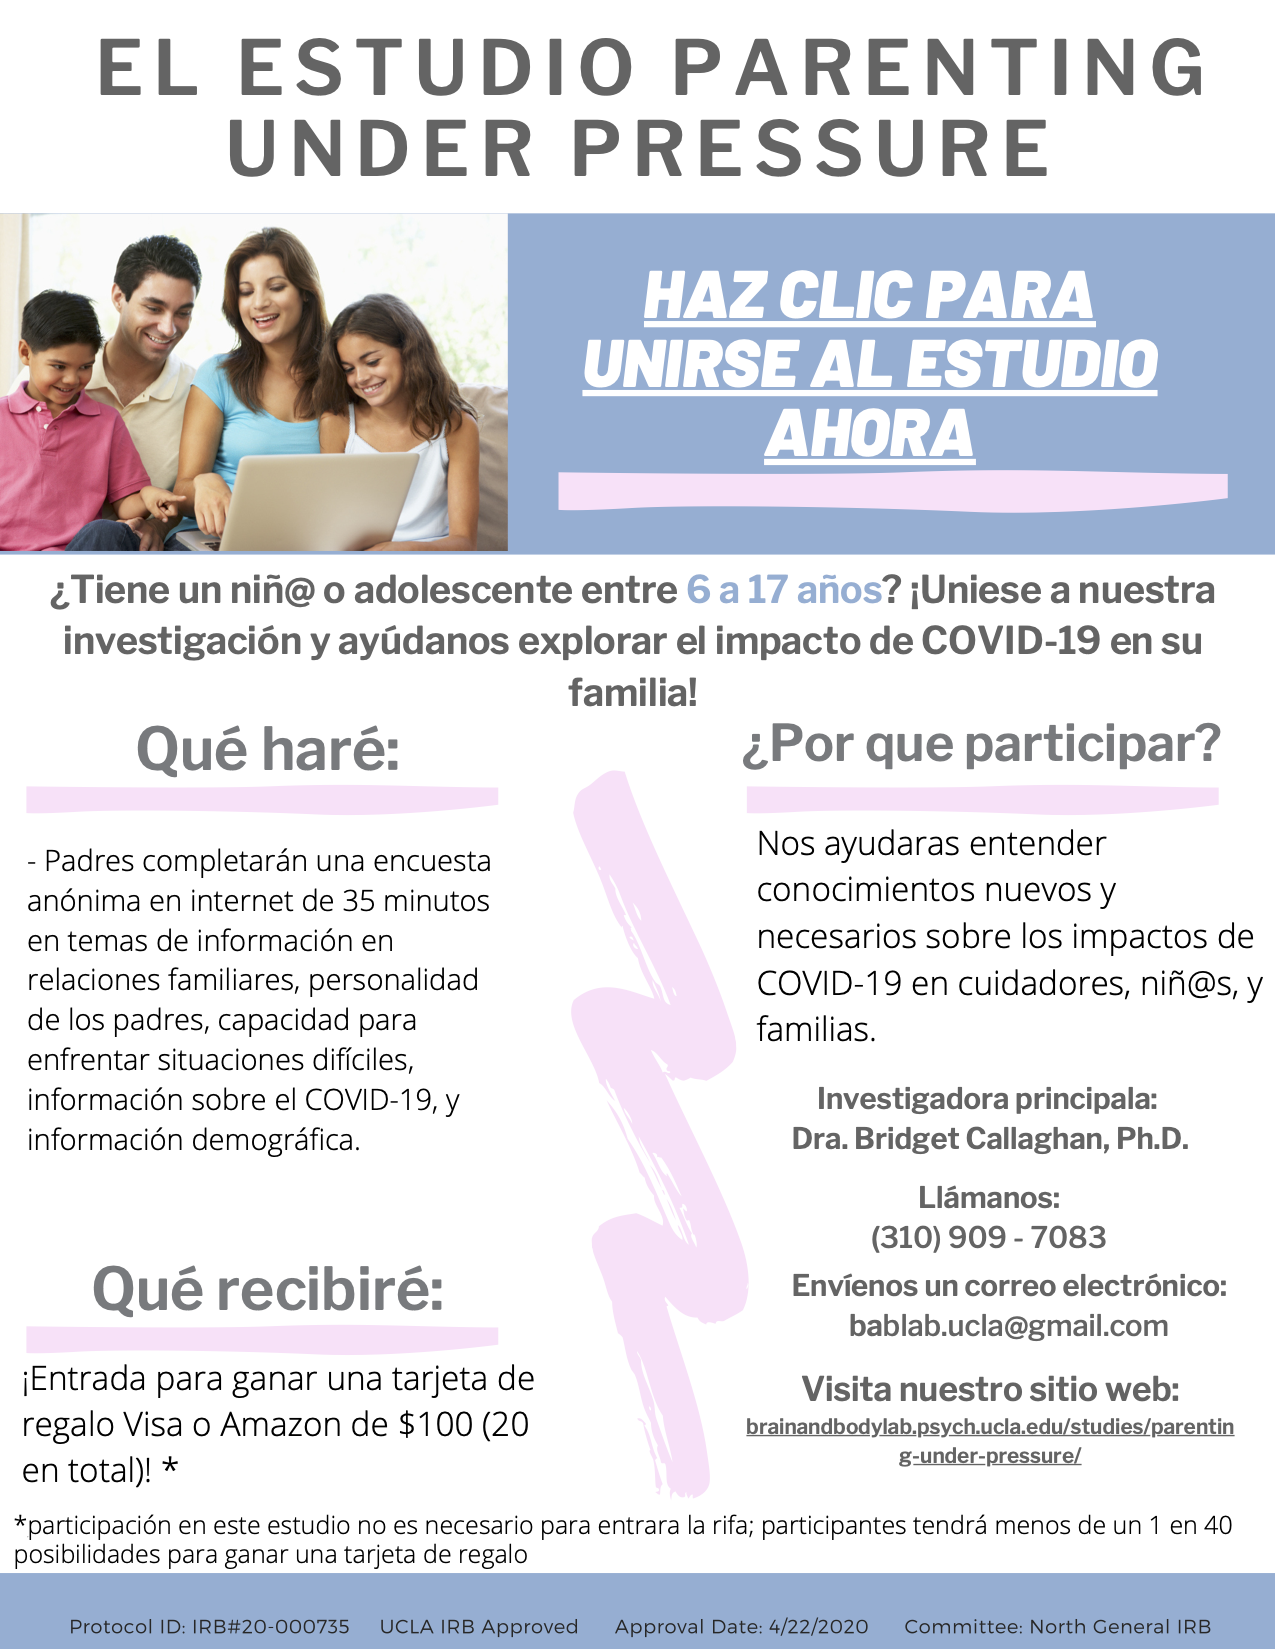
\includegraphics{images/PUP_spanish_flyer.png}
\caption{}
\end{figure}

\begin{center}\rule{0.5\linewidth}{0.5pt}\end{center}

\hypertarget{timing}{%
\subsection{Timing}\label{timing}}

PUP 1 took approximately 60 minutes to complete, including 5 minutes of child self-report following the Written Response COVID-19 prompt. PUP 2 was shortened to approximately 35 minutes and did not include a qualitative written section.

\begin{center}\rule{0.5\linewidth}{0.5pt}\end{center}

\hypertarget{pup-1-questionnaire-order}{%
\subsection{PUP 1 Questionnaire Order}\label{pup-1-questionnaire-order}}

\begin{enumerate}
\def\labelenumi{\arabic{enumi}.}
\tightlist
\item
  Participant
\item
  COVID-19 Information
\item
  FIVE
\item
  SOI
\item
  GMF
\item
  PCRQ
\item
  PSCQ
\item
  BIQ
\item
  PBQ
\item
  TESI
\item
  Demographics
\item
  STAI
\item
  RCADS
\item
  PANAS (Pre- assessment)
\item
  Parental Written Response
\item
  PANAS (Post- assessment)
\item
  Child Written Response
  (if applicable, \#18-20)
\item
  Child \#2 Written Response
\item
  Child \#3 Written Response
\item
  Child \#4 Written Response
\item
  Resources
\end{enumerate}

\begin{center}\rule{0.5\linewidth}{0.5pt}\end{center}

\hypertarget{pup-2-questionnaire-order}{%
\subsection{PUP 2 Questionnaire Order}\label{pup-2-questionnaire-order}}

\begin{enumerate}
\def\labelenumi{\arabic{enumi}.}
\tightlist
\item
  Participant
\item
  Information
\item
  FIVE
\item
  SOI
\item
  PCRQ
\item
  BIQ
\item
  PBQ
\item
  Demographics
\item
  Resources
\end{enumerate}

\begin{center}\rule{0.5\linewidth}{0.5pt}\end{center}

\hypertarget{pup-1-attention-checks}{%
\subsection{PUP 1 Attention Checks}\label{pup-1-attention-checks}}

\begin{enumerate}
\def\labelenumi{\arabic{enumi}.}
\tightlist
\item
  FIVE
\item
  PCRQ
\item
  PBQ
\item
  TESI
\item
  RCADS
\end{enumerate}

\begin{center}\rule{0.5\linewidth}{0.5pt}\end{center}

\hypertarget{pup-2-attention-checks}{%
\subsection{PUP 2 Attention Checks}\label{pup-2-attention-checks}}

\begin{enumerate}
\def\labelenumi{\arabic{enumi}.}
\tightlist
\item
  FIVE
\item
  PCRQ
\item
  PBQ
\end{enumerate}

\begin{center}\rule{0.5\linewidth}{0.5pt}\end{center}

\hypertarget{analysis}{%
\chapter{Analysis}\label{analysis}}

\hypertarget{mixed-methods}{%
\section{Mixed Methods}\label{mixed-methods}}

\hypertarget{preregistration}{%
\subsection{Preregistration}\label{preregistration}}

\begin{figure}
\centering

\includegraphics{images/qual_preregistration_QR.png}
\caption{}
\end{figure}

\hypertarget{preprint}{%
\subsection{Preprint}\label{preprint}}

\begin{figure}
\centering

\includegraphics{images/qual_preprint_QR.png}
\caption{}
\end{figure}

\begin{center}\rule{0.5\linewidth}{0.5pt}\end{center}

\hypertarget{references}{%
\chapter{References}\label{references}}

Adler, N. E., Epel, E. S., Castellazzo, G., \& Ickovics, J. R. (2000).
Relationship of subjective and objective social status with psychological
and physiological functioning:Preliminary data in healthy, White women.
Health Psychology, 19(6), 586-592.

Biringen, Z., Robinson, J. \& Emde, R. (1998). The Emotional Availability
Scales (3rd ed.). Retrieved from www.emotionalavailability.com

Berry, J. O., \& Jones, W. H. (1995). The Parental Stress Scale: Initial
psychometric evidence. Journal of Social and Personal Relationships, 12,
463-472.

Cheng, C., \& Cheung, M. W. (2005). Psychological responses to outbreak of
severe acute respiratory syndrome: a prospective, multiple time‐point
study. Journal of Personality, 73(1), 261-285.

Chorpita, B. F., Yim, L., Moffitt, C., Umemoto, L. A., \& Francis, S. E. (2000). Assessment of
symptoms of DSM-IV anxiety and depression in children: A revised child anxiety and
depression scale. Behaviour research and therapy, 38(8), 835-855.

Chrisman, A. K., \& Dougherty, J. G. (2014). Mass trauma: Disasters, terrorism, and war. Child
and Adolescent Psychiatric Clinics, 23(2), 257-279.

Ehenreich-May, J. (2020). Fear of Illness and Virus Evaluation (FIVE) -- Parent Report Form
{[}Measurement instrument{]}. Retrieved from
\url{https://drive.google.com/drive/u/0/folders/1RhHt77XQzItmpw_yGAteILlMNIGpj5pU}

Ehenreich-May, J. (2020). Fear of Illness and Virus Evaluation (FIVE) -- Adult Report Form
{[}Measurement instrument{]}. Retrieved from
\url{https://drive.google.com/drive/u/0/folders/1RhHt77XQzItmpw_yGAteILlMNIGpj5pU}

Furman W, Buhrmester D. The Network of Relationships Inventory: Behavioral Systems
Version. Int J Behav Dev. 2009;33(5):470--478. \url{doi:10.1177/0165025409342634}

Gewirtz, A., Forgatch, M., \& Wieling, E. (2008). Parenting practices as potential mechanisms for
child adjustment following mass trauma. Journal of Marital and Family Therapy, 34(2),
177-192.

Grant, M.L. \& Kothare, S. (2005). Older Child/Adolescent Sleep Habits Questionnaire- Parent
Report {[}Measurement instrument{]}. Retrieved from \url{http://www.childrenshospital.org/-}
/media/Centers-and-Services/Programs/O\_Z/Pediatric-Sleep-Disorders-Center/Research-
VersionParentsAdolescentSHQLC.ashx?la=en\&hash=2CAB880BC93A221FB31BD6BA
DE3C7B6313D139AB

Guimond, A. B., Wilcox, M. J., \& Lamorey, S. G. (2008). The early intervention parenting self-
Efficacy Scale (EIPSES) scale construction and initial psychometric evidence. Journal of
early intervention, 30(4), 295-320.

Ladouceur, C.D. (2020). COVID-19 Adolescent Symptom \& Psychological Experience (CASPE)-
Parent Questionnaire {[}Measurement instrument{]}. Retrieved from \url{https://osf.io/hu2k9/}

Luyten, P., Mayes, L. C., Nijssens, L., \& Fonagy, P. (2017). The parental reflective functioning
questionnaire: Development and preliminary validation. PLOS ONE, 12(5), e0176218.
doi: 10.1371/journal.pone.0176218

Ollendick, T. H. (1983). Reliability and validity of the revised fear survey schedule for children
(FSSC-R). Behaviour research and therapy, 21(6), 685-692.

Owens, J. A., Spirito, A., \& McGuinn, M. (2000). The Children's Sleep Habits Questionnaire
(CSHQ): psychometric properties of a survey instrument for school-aged children. Sleep-
New York-, 23(8), 1043-1052.

Pennebaker, J. W. (1997). Writing about emotional experiences as a therapeutic
process. Psychological science, 8(3), 162-166.

Pereira, A. I., Barros, L., Roberto, M. S., \& Marques, T. (2017). Development of the Parent
Emotion Regulation Scale (PERS): Factor Structure and Psychometric Qualities. Journal
of Child and Family Studies, 26(12), 3327-3338.

Perrin, P. C., McCabe, O. L., Everly, G. S., \& Links, J. M. (2009). Preparing for an influenza
pandemic: mental health considerations. Prehospital and disaster medicine, 24(3), 223-
230.

Pfefferbaum, B. J., Devoe, E. R., Stuber, J., Schiff, M., Klein, T. P., \& Fairbrother, G. (2005).
Psychological impact of terrorism on children and families in the United States. Journal
of aggression, maltreatment \& trauma, 9(3-4), 305-317.

Pfiefer, J. (2020). Adolescent Social Connection \& Coping During COVID Questionnaire (ASC)
{[}Measurement instrument{]}. Retrieved from \url{https://osf.io/jakg5/}

Pfiefer, J. (2020). Combined COVID Health Emotional Lifestyle Changes{[}Measurement
instrument{]}. Retri{]}. Retrieved from \url{https://osf.io/c2z8k/}

Pfiefer, J. (2020). COVID Lifestyle Changes {[}Measurement instrument{]}. Retrieved from
\url{https://osf.io/wqmda/}

Pfiefer, J. \& Lewis, J. (2020). Modified KidCOPE {[}Measurement instrument{]}. Retrieved from
\url{https://osf.io/wcgj8/}

Phillips, D., Scheibelhut, L., \& Prince, S. (2003, April). Children's responses to the terrorist
attacks of September 11th: An exploratory study. In J. Lawrence Aber \& D. Phillips
(Chairs), The aftermath of September 11th, 2001: Developmental effects and policy
implications. Symposium conducted at the Biennial Meetings of the Society for Research
in Child Development, Tampa, FL.
Pianta, R.C. (1992). Child-Preant Relationship Scale (CPRS) {[}Measurement instrument{]}.
Retrieved from ttps://curry.virginia.edu/faculty-research/centers-labs-
projects/castl/measures-developed-robert-c-pianta-phd

Remmerswaal, D., \& Muris, P. (2011). Children's fear reactions to the 2009 Swine Flu
pandemic: The role of threat information as provided by parents. Journal of anxiety
disorders, 25(3), 444-449.

Svebak, S. (1993). The development of the tension and effort stress inventory (TESI). Advances
in reversal theory, 189-204.

Waters, E. (1995). Appendix A: The attachment Q-set (version 3.0). Monographs of the society
for research in child development, 234-246.

Watson, D., Clark, L. A., \& Tellegen, A. (1988). Development and validation of brief measures
of positive and negative affect: the PANAS scales. Journal of personality and social
psychology, 54(6), 1063.

Wu, K. K., Chan, S. K., \& Ma, T. M. (2005). Posttraumatic stress, anxiety, and depression in
survivors of severe acute respiratory syndrome (SARS). Journal of Traumatic Stress:
Official Publication of The International Society for Traumatic Stress Studies, 18(1), 39-
42.

\hypertarget{contributions}{%
\chapter{Contributions}\label{contributions}}

\hypertarget{general}{%
\section{General}\label{general}}

\begin{longtable}[]{@{}ll@{}}
\toprule
\begin{minipage}[b]{0.22\columnwidth}\raggedright
Name\strut
\end{minipage} & \begin{minipage}[b]{0.72\columnwidth}\raggedright
Role\strut
\end{minipage}\tabularnewline
\midrule
\endhead
\begin{minipage}[t]{0.22\columnwidth}\raggedright
Bridget Callaghan\strut
\end{minipage} & \begin{minipage}[t]{0.72\columnwidth}\raggedright
Study conception, design, planning, supervision\strut
\end{minipage}\tabularnewline
\begin{minipage}[t]{0.22\columnwidth}\raggedright
Kristen Chu\strut
\end{minipage} & \begin{minipage}[t]{0.72\columnwidth}\raggedright
Study conception, design, planning, implementation, data cleaning, data analysis, documentation creation\strut
\end{minipage}\tabularnewline
\begin{minipage}[t]{0.22\columnwidth}\raggedright
Chloe Schwartz\strut
\end{minipage} & \begin{minipage}[t]{0.72\columnwidth}\raggedright
Study conception, Design, planning, implementation, data cleaning, data analysis, documentation creation\strut
\end{minipage}\tabularnewline
\begin{minipage}[t]{0.22\columnwidth}\raggedright
Emily Towner\strut
\end{minipage} & \begin{minipage}[t]{0.72\columnwidth}\raggedright
Study conception, design, planning, implementation, data cleaning, data analysis\strut
\end{minipage}\tabularnewline
\begin{minipage}[t]{0.22\columnwidth}\raggedright
Grant Grech\strut
\end{minipage} & \begin{minipage}[t]{0.72\columnwidth}\raggedright
Study translation, piloting, REDCap questionnaire entry, recruitment\strut
\end{minipage}\tabularnewline
\begin{minipage}[t]{0.22\columnwidth}\raggedright
Daisy Ramirez\strut
\end{minipage} & \begin{minipage}[t]{0.72\columnwidth}\raggedright
Study translation, piloting, REDCap questionnaire entry, recruitment\strut
\end{minipage}\tabularnewline
\begin{minipage}[t]{0.22\columnwidth}\raggedright
Nicole Fonacier\strut
\end{minipage} & \begin{minipage}[t]{0.72\columnwidth}\raggedright
Study translation, piloting, REDCap questionnaire entry, recruitment\strut
\end{minipage}\tabularnewline
\begin{minipage}[t]{0.22\columnwidth}\raggedright
Aileen Gozali\strut
\end{minipage} & \begin{minipage}[t]{0.72\columnwidth}\raggedright
Implementation, piloting\strut
\end{minipage}\tabularnewline
\begin{minipage}[t]{0.22\columnwidth}\raggedright
Danielle Ladensack\strut
\end{minipage} & \begin{minipage}[t]{0.72\columnwidth}\raggedright
Implementation, piloting\strut
\end{minipage}\tabularnewline
\begin{minipage}[t]{0.22\columnwidth}\raggedright
Ananya Eervani\strut
\end{minipage} & \begin{minipage}[t]{0.72\columnwidth}\raggedright
Study translation\strut
\end{minipage}\tabularnewline
\begin{minipage}[t]{0.22\columnwidth}\raggedright
Alyssa Wieand\strut
\end{minipage} & \begin{minipage}[t]{0.72\columnwidth}\raggedright
REDCap questionnaire entry\strut
\end{minipage}\tabularnewline
\begin{minipage}[t]{0.22\columnwidth}\raggedright
Reese Wix\strut
\end{minipage} & \begin{minipage}[t]{0.72\columnwidth}\raggedright
REDCap questionnaire entry\strut
\end{minipage}\tabularnewline
\begin{minipage}[t]{0.22\columnwidth}\raggedright
Alyssa Ortega\strut
\end{minipage} & \begin{minipage}[t]{0.72\columnwidth}\raggedright
REDCap questionnaire entry\strut
\end{minipage}\tabularnewline
\begin{minipage}[t]{0.22\columnwidth}\raggedright
Michael To\strut
\end{minipage} & \begin{minipage}[t]{0.72\columnwidth}\raggedright
REDCap questionnaire entry\strut
\end{minipage}\tabularnewline
\bottomrule
\end{longtable}

\begin{center}\rule{0.5\linewidth}{0.5pt}\end{center}

\hypertarget{projectspapers}{%
\section{Projects/Papers}\label{projectspapers}}

\hypertarget{pup-mixed-methods}{%
\subsection{PUP Mixed Methods}\label{pup-mixed-methods}}

\begin{longtable}[]{@{}ll@{}}
\toprule
\begin{minipage}[b]{0.22\columnwidth}\raggedright
Name\strut
\end{minipage} & \begin{minipage}[b]{0.72\columnwidth}\raggedright
Role\strut
\end{minipage}\tabularnewline
\midrule
\endhead
\begin{minipage}[t]{0.22\columnwidth}\raggedright
Bridget Callaghan\strut
\end{minipage} & \begin{minipage}[t]{0.72\columnwidth}\raggedright
Supervision, data analysis, writing, editing\strut
\end{minipage}\tabularnewline
\begin{minipage}[t]{0.22\columnwidth}\raggedright
Kristen Chu\strut
\end{minipage} & \begin{minipage}[t]{0.72\columnwidth}\raggedright
Data analysis, writing, editing, preregistration, ISDP 2020 Poster\strut
\end{minipage}\tabularnewline
\begin{minipage}[t]{0.22\columnwidth}\raggedright
Chloe Schwartz\strut
\end{minipage} & \begin{minipage}[t]{0.72\columnwidth}\raggedright
Data analysis, editing\strut
\end{minipage}\tabularnewline
\begin{minipage}[t]{0.22\columnwidth}\raggedright
Emily Towner\strut
\end{minipage} & \begin{minipage}[t]{0.72\columnwidth}\raggedright
Data analysis\strut
\end{minipage}\tabularnewline
\bottomrule
\end{longtable}

\hypertarget{pup-quantitative}{%
\subsection{PUP Quantitative}\label{pup-quantitative}}

\begin{longtable}[]{@{}ll@{}}
\toprule
\begin{minipage}[b]{0.22\columnwidth}\raggedright
Name\strut
\end{minipage} & \begin{minipage}[b]{0.72\columnwidth}\raggedright
Role\strut
\end{minipage}\tabularnewline
\midrule
\endhead
\begin{minipage}[t]{0.22\columnwidth}\raggedright
Bridget Callaghan\strut
\end{minipage} & \begin{minipage}[t]{0.72\columnwidth}\raggedright
Supervision, writing, editing\strut
\end{minipage}\tabularnewline
\begin{minipage}[t]{0.22\columnwidth}\raggedright
Chloe Schwartz\strut
\end{minipage} & \begin{minipage}[t]{0.72\columnwidth}\raggedright
Data analysis, writing, editing preregistration, ISDP 2020 Poster\strut
\end{minipage}\tabularnewline
\begin{minipage}[t]{0.22\columnwidth}\raggedright
Kristen Chu\strut
\end{minipage} & \begin{minipage}[t]{0.72\columnwidth}\raggedright
Data analysis, editing\strut
\end{minipage}\tabularnewline
\begin{minipage}[t]{0.22\columnwidth}\raggedright
Emily Towner\strut
\end{minipage} & \begin{minipage}[t]{0.72\columnwidth}\raggedright
Data analysis\strut
\end{minipage}\tabularnewline
\bottomrule
\end{longtable}

\begin{center}\rule{0.5\linewidth}{0.5pt}\end{center}

\bibliography{book.bib,packages.bib,ref.bib}

\end{document}
